%----------
%   IMPORTANTE
%----------

% Si nunca has utilizado LaTeX es conveniente que aprendas una serie de conceptos básicos antes de utilizar esta plantilla. Te aconsejamos que leas previamente algún tutorial (puedes encontar muchos en Internet).

% Esta plantilla está basada en las recomendaciones de la guía "Trabajo fin de Máster: Escribir el TFM", que encontrarás en http://uc3m.libguides.com/TFM/escribir
% contiene recomendaciones de la Biblioteca basadas principalmente en estilos APA e IEEE, pero debes seguir siempre las orientaciones de tu Tutor de TFM y la normativa de TFM para tu titulación.

% Encontrarás un ejemplo de TFM realizado con esta misma plantilla en la carpeta "_ejemplo_TFM_2019". Consúltalo porque contiene ejemplos útiles para incorporar tablas, figuras, listados de código, bibliografía, etc.



%----------
%	CONFIGURACIÓN DEL DOCUMENTO
%----------

% Definimos las características del documento y añadimos una serie de paquetes (\usepackage{package}) que agregan funcionalidades a LaTeX.

\documentclass[12pt]{report} %fuente a 12pt

%------------------------------------------------------------------------------------


\hyphenation{ciber-delincuentes pro-por-cionadas com-pro-meter ges-tio-nar la-bo-ra-torio net-working pro-por-cio-na-do cen-tra-li-za-da im-ple-men-ta-do he-rra-mien-tas in-fra-es-truc-tu-ra Di-rec-to-ry im-ple-men-ta-cio-nes auten-ti-ca-cion u-ti-li-za-dos} 
\PassOptionsToPackage{hyphens}{url}
\usepackage{float}

\usepackage{cite}


\usepackage{color}
\definecolor{gray97}{gray}{.97}
\definecolor{gray75}{gray}{.75}
\definecolor{gray45}{gray}{.45}

\usepackage{listings}
\lstset{ frame=Ltb,
framerule=0pt,
aboveskip=0.5cm,
framextopmargin=3pt,
framexbottommargin=3pt,
framexleftmargin=0.4cm,
framesep=0pt,
rulesep=.4pt,
backgroundcolor=\color{gray97},
rulesepcolor=\color{black},
%
stringstyle=\ttfamily,
showstringspaces = false,
basicstyle=\small\ttfamily,
commentstyle=\color{gray45},
keywordstyle=\bfseries,
%
numbers=left,
numbersep=15pt,
numberstyle=\tiny,
numberfirstline = false,
breaklines=true,
}

% minimizar fragmentado de listados
\lstnewenvironment{listing}[1][]
{\lstset{#1}\pagebreak[0]}{\pagebreak[0]}

\lstdefinestyle{consola}
{basicstyle=\scriptsize\bf\ttfamily,
backgroundcolor=\color{gray75},
}

\lstdefinestyle{C}
{language=C,
}

%------------------------------------------------------------------------------------



% MÁRGENES: 2,5 cm sup. e inf.; 3 cm izdo. y dcho.
\usepackage[
a4paper,
vmargin=2.5cm,
hmargin=3cm
]{geometry}

% INTERLINEADO: Estrecho (6 ptos./interlineado 1,15) o Moderado (6 ptos./interlineado 1,5)
\renewcommand{\baselinestretch}{1.15}
\parskip=6pt

% DEFINICIÓN DE COLORES para portada y listados de código
\usepackage[table]{xcolor}
\definecolor{azulUC3M}{RGB}{0,0,102}
\definecolor{gray97}{gray}{.97}
\definecolor{gray75}{gray}{.75}
\definecolor{gray45}{gray}{.45}

% Soporte para GENERAR PDF/A --es importante de cara a su inclusión en e-Archivo porque es el formato óptimo de preservación y a la generación de metadatos, tal y como se describe en http://uc3m.libguides.com/ld.php?content_id=31389625. En la carpeta incluímos el archivo plantilla_tfg_2017.xmpdata en el que puedes incluir los metadatos que se incorporarán al archivo PDF cuando lo compiles. Ese archivo debe llamarse igual que tu archivo .tex. Puedes ver un ejemplo en esta misma carpeta.
\usepackage[a-1b]{pdfx}

% ENLACES
\usepackage{hyperref}
\hypersetup{colorlinks=true,
	linkcolor=black, % enlaces a partes del documento (p.e. índice) en color negro
	urlcolor=blue} % enlaces a recursos fuera del documento en azul

% EXPRESIONES MATEMATICAS
\usepackage{amsmath,amssymb,amsfonts,amsthm}

\usepackage{txfonts} 
\usepackage[T1]{fontenc}
\usepackage[utf8]{inputenc}

\usepackage[spanish, es-tabla]{babel} 
\usepackage[babel, spanish=spanish]{csquotes}
\AtBeginEnvironment{quote}{\small}

% diseño de PIE DE PÁGINA
\usepackage{fancyhdr}
\pagestyle{fancy}
\fancyhf{}
\renewcommand{\headrulewidth}{0pt}
\rfoot{\thepage}
\fancypagestyle{plain}{\pagestyle{fancy}}

% DISEÑO DE LOS TÍTULOS de las partes del trabajo (capítulos y epígrafes o subcapítulos)
\usepackage{titlesec}
\usepackage{titletoc}

\titleformat{\chapter}[block]
{\large\bfseries} %\filcenter}
{\thechapter.}
{5pt}
{}
{}
\titlespacing{\chapter}{0pt}{0pt}{*3}
\titlecontents{chapter}
[0pt]                                               
{}
{\contentsmargin{0pt}\thecontentslabel.\enspace}
{\contentsmargin{0pt}}                        
{\titlerule*[.7pc]{.}\contentspage}                 

\titleformat{\section}
{\bfseries}
{\thesection.}
{5pt}
{}
\titlecontents{section}
[5pt]                                               
{}
{\contentsmargin{0pt}\thecontentslabel.\enspace}
{\contentsmargin{0pt}}
{\titlerule*[.7pc]{.}\contentspage}

\titleformat{\subsection}
{\normalsize\bfseries}
{\thesubsection.}
{5pt}
{}
\titlecontents{subsection}
[10pt]                                               
{}
{\contentsmargin{0pt}                          
	\thecontentslabel.\enspace}
{\contentsmargin{0pt}}                        
{\titlerule*[.7pc]{.}\contentspage}  


% DISEÑO DE TABLAS. Puedes elegir entre el estilo para ingeniería o para ciencias sociales y humanidades. Por defecto, está activado el estilo de ingeniería. Si deseas utilizar el otro, comenta las líneas del diseño de ingeniería y descomenta las del diseño de ciencias sociales y humanidades
\usepackage{multirow} % permite combinar celdas 
\usepackage{caption} % para personalizar el título de tablas y figuras
% \usepackage{floatrow} % utilizamos este paquete y sus macros \ttabbox y \ffigbox para alinear los nombres de tablas y figuras de acuerdo con el estilo definido. Para su uso ver archivo de ejemplo 
\usepackage{array} % con este paquete podemos definir en la siguiente línea un nuevo tipo de columna para tablas: ancho personalizado y contenido centrado
\newcolumntype{P}[1]{>{\centering\arraybackslash}p{#1}}
\DeclareCaptionFormat{upper}{#1#2\uppercase{#3}\par}

% Diseño de tabla para ingeniería
\captionsetup[table]{
	format=upper,
	name=TABLA,
	justification=centering,
	labelsep=period,
	width=.75\linewidth,
	labelfont=small,
	font=small,
}

%Diseño de tabla para ciencias sociales y humanidades
%\captionsetup[table]{
%	justification=raggedright,
%	labelsep=period,
%	labelfont=small,
%	singlelinecheck=false,
%	font={small,bf}
%}


% DISEÑO DE FIGURAS. Puedes elegir entre el estilo para ingeniería o para ciencias sociales y humanidades. Por defecto, está activado el estilo de ingeniería. Si deseas utilizar el otro, comenta las líneas del diseño de ingeniería y descomenta las del diseño de ciencias sociales y humanidades
\usepackage{graphicx}
\graphicspath{{imagenes/}} %ruta a la carpeta de imágenes

% Diseño de figuras para ingeniería
\captionsetup[figure]{
	format=hang,
	name=Fig.,
	singlelinecheck=off,
	labelsep=period,
	labelfont=small,
	font=small		
}

% Diseño de figuras para ciencias sociales y humanidades
%\captionsetup[figure]{
%	format=hang,
%	name=Figura,
%	singlelinecheck=off,
%	labelsep=period,
%	labelfont=small,
%	font=small		
%}


% NOTAS A PIE DE PÁGINA
\usepackage{chngcntr} %para numeración contínua de las notas al pie
\counterwithout{footnote}{chapter}

% LISTADOS DE CÓDIGO
% soporte y estilo para listados de código. Más información en https://es.wikibooks.org/wiki/Manual_de_LaTeX/Listados_de_código/Listados_con_listings
\usepackage{listings}

% definimos un estilo de listings
\lstdefinestyle{estilo}{ frame=Ltb,
	framerule=0pt,
	aboveskip=0.5cm,
	framextopmargin=3pt,
	framexbottommargin=3pt,
	framexleftmargin=0.4cm,
	framesep=0pt,
	rulesep=.4pt,
	backgroundcolor=\color{gray97},
	rulesepcolor=\color{black},
	%
	basicstyle=\ttfamily\footnotesize,
	keywordstyle=\bfseries,
	stringstyle=\ttfamily,
	showstringspaces = false,
	commentstyle=\color{gray45},     
	%
	numbers=left,
	numbersep=15pt,
	numberstyle=\tiny,
	numberfirstline = false,
	breaklines=true,
	xleftmargin=\parindent
}

\captionsetup[lstlisting]{font=small, labelsep=period}
% fijamos el estilo a utilizar 
\lstset{style=estilo}
\renewcommand{\lstlistingname}{\uppercase{Código}}


%BIBLIOGRAFÍA - PUEDES ELEGIR ENTRE ESTILO IEEE O APA. POR DEFECTO ESTÁ CONFIGURADO IEEE. SI DESEAS USAR APA, COMENTA LAS LÍNEA DE IEEE Y DESCOMENTA LAS DE APA. Si haces cambios en la configuración de la bibliografía y no obtienes los resultados esperados, es recomendable limpiar los archivos auxiliares y volver a compilar en este orden: COMPILAR-BIBLIOGRAFIA-COMPILAR

% Tienes más información sobre cómo generar bibliografía y CONFIGURAR TU EDITOR DE TEXTO para compilar con biber en http://tex.stackexchange.com/questions/154751/biblatex-with-biber-configuring-my-editor-to-avoid-undefined-citations , https://www.overleaf.com/learn/latex/Bibliography_management_in_LaTeX y en http://www.ctan.org/tex-archive/macros/latex/exptl/biblatex-contrib
% También te recomendamos consultar la guía temática de la Biblioteca sobre citas bibliográficas: http://uc3m.libguides.com/guias_tematicas/citas_bibliograficas/inicio

% CONFIGURACIÓN PARA LA BIBLIOGRAFÍA IEEE
% \usepackage[backend=biber, style=ieee, isbn=false,sortcites, maxbibnames=5, minbibnames=1]{biblatex} % Configuración para el estilo de citas de IEEE, recomendado para el área de ingeniería. "maxbibnames" indica que a partir de 5 autores trunque la lista en el primero (minbibnames) y añada "et al." tal y como se utiliza en el estilo IEEE.

%CONFIGURACIÓN PARA LA BIBLIOGRAFÍA APA
%\usepackage[style=apa, backend=biber, natbib=true, hyperref=true, uniquelist=false, sortcites]{biblatex}
%\DeclareLanguageMapping{spanish}{spanish-apa}

% Añadimos las siguientes indicaciones para mejorar la adaptación de los estilos en español
% \DefineBibliographyStrings{spanish}{%
% 	andothers = {et\addabbrvspace al\adddot}
% }
% \DefineBibliographyStrings{spanish}{
% 	url = {\adddot\space[En línea]\adddot\space Disponible en:}
% }
% \DefineBibliographyStrings{spanish}{
% 	urlseen = {Acceso:}
% }
% \DefineBibliographyStrings{spanish}{
% 	pages = {pp\adddot},
% 	page = {p.\adddot}
% }

% \addbibresource{Bibliografia/Bibliografia.bib} % llama al archivo bibliografia.bib en el que debería estar la bibliografía utilizada


%-------------
%	DOCUMENTO
%-------------

\begin{document}
\pagenumbering{roman} % Se utilizan cifras romanas en la numeración de las páginas previas al cuerpo del trabajo
	

%----------
%	PORTADA
%----------	

\thispagestyle{empty}


%----------
%	PORTADA
%----------	
\begin{titlepage}
	\begin{sffamily}
	\color{azulUC3M}
	\begin{center}
		\begin{figure}[H] %incluimos el logotipo de la Universidad
			\makebox[\textwidth][c]{
\includegraphics[width=16cm]{Portada_Logo.png}}
		\end{figure}
		\vspace{1cm}
		\begin{Large}
			Máster Universitario en Ciberseguridad\\			
			2018-2019\\
			\vspace{1cm}		
			\textsl{Trabajo Fin de Máster}
			\bigskip
			
		\end{Large}
		 	% {\Huge ``CIBEREJERCICIOS PARA EVALUAR ACTIVE DIRECTORY EN SUS DISTINTAS VERSIONES. ''}\\
		 	{\Huge ``Ciberejercicios para evaluar \\
		 	Active Directory en sus distinas versiones. ''}\\
		 	\vspace*{0.5cm}
	 		\rule{10.5cm}{0.1mm}\\
			\vspace*{0.9cm}
			{\LARGE Borja Lorenzo Fernádez}\\ 
			\vspace*{1cm}
		\begin{Large}
			Tutor\\
			Andrés Marín López\\
		\end{Large}
	\end{center}
	
	\vfill
	\color{black}
	\begin{footnotesize}
	\noindent\fbox{
	\begin{minipage}{\textwidth}
		\textbf{DETECCIÓN DEL PLAGIO}\\
		La Universidad utiliza el programa \textbf{Turnitin Feedback Studio} para comparar la originalidad del trabajo entregado por cada estudiante con millones de recursos electrónicos y detecta aquellas partes del texto copiadas y pegadas. Copiar o plagiar en un TFM es considerado una \textbf{\underline{Falta Grave}}, y puede conllevar la expulsión definitiva de la Universidad.
	\end{minipage}	
	}
	% \vspace*{.5cm}\\	
	% \noindent
\includegraphics[width=4.2cm]{imagenes/creativecommons.png}\\
	% \emph{[Incluir en el caso del interés en su publicación en el archivo abierto]}\\
	% Esta obra se encuentra sujeta a la licencia Creative Commons \textbf{Reconocimiento - No Comercial - Sin Obra Derivada}

	\end{footnotesize}
	\end{sffamily}
\end{titlepage}

\newpage %página en blanco o de cortesía
\thispagestyle{empty}
\mbox{}

%----------
%	Agracedimientos
%----------	
\chapter*{Agradecimientos}
%----------
%	Agracedimientos
%----------	

\setcounter{page}{3}
	
	% ESCRIBIR LA DEDICATORIA AQUÍ	


En primer lugar, me gustaría dedicar este trabajo a mis abuelos ya que sin ellos no habría podido llegar a donde he llegado. \\

Agradecer especialmente a mi familia, padres y hermanos por ayudarme y aguantarme incluso en los peores momentos. \\

Quiero agradecer a María, por la dedicación, el esfuerzo y la paciencia que ha tenido conmigo y por habeme enseñado tanto y haberme facilitado las cosas para llegar hasta aquí. \\

Por último, agradecer a todos los que me han ayudado con el desarrollo de este proyecto desinteresadamente, especialemente a Atl4s, Arcocapaz, Cynops y Mamatb.
\vfill
\newpage %página en blanco o de cortesía
\thispagestyle{empty}
\mbox{}


%----------
%	RESUMEN Y PALABRAS CLAVE
%----------	
\chapter*{Resumen}
%----------
%	RESUMEN Y PALABRAS CLAVE
%----------	

\setcounter{page}{5}
	
Active Directory (AD) es una base de datos distribuida que permite a los administradores gestionar de manera eficiente la información de la empresa y los límites de la misma. En la actualidad, Active Directory es considerado una de las partes fundamentales para el correcto funcionamiento de cualquier empresa. La información gestionada por Active Directory, engloba usuarios, clientes, proveedores, dispositivos (ordenadores, servidores, impresoras...), servicios y aplicaciones así como la interacción entre ellos. Por lo tanto, supone uno de los principales objetivos para atacantes y ciberdelincuentes así como una gran problema de seguridad para una organización si el sistema de gestión principal se ve comprometido. En los últimos años se ha producido un gran aumento de ataques contra Active Directory cuyo objetivo es hacerse con el control de la empresa y comprometer la seguridad de la información, esto es debido a que se han perfeccionado los principales ataques así como la implementación de nuevas herramientas que facilitan todo tipo de ataques. \\

Con el fin de contribuir al desarrollo y mejora de la seguridad de Active Directory y por ende, de las empresas y particulares que hacen uso de ello, el trabajo realizado se centra en el estudio de los principales componentes que engloban la seguridad y gestión del sistema de directorio Active Directory a través de la creación de un laboratorio, de manera local, y el análisis y revisión de los principales ataques y amenazas usadas en la actualidad para vulnerar dicho sistema de gestión. Para ello, se implementa una topología que simula una empresa ficticia e implementa la última versión de Windows Server 2019.\\ 

\textit{\textbf{Palabras Clave:}}

Microsoft Active Directory, Domain Controller, Kerberos, Ciberseguridad, Windows Server, Pentesting, Red Team
	
		
\vfill
\newpage %página en blanco o de cortesía
\thispagestyle{empty}
\mbox{}






	

%-------------------------------------------------------------------------------
%	ÍNDICES
%-------------------------------------------------------------------------------

%--
%Índice general
%-
\tableofcontents
\thispagestyle{fancy}

\newpage %página en blanco o de cortesía
\thispagestyle{empty}
\mbox{}

%--
%Índice de figuras. Si no se incluyen, comenta las líneas siguientes
%-
\listoffigures
\thispagestyle{fancy}

\newpage %página en blanco o de cortesía
\thispagestyle{empty}
\mbox{}

%--
%Índice de tablas. Si no se incluyen, comenta las líneas siguientes
%-
\listoftables
\thispagestyle{fancy}

\newpage %página en blanco o de cortesía
\thispagestyle{empty}
\mbox{}


%-------------------------------------------------------------------------------
%-------------------------------------------------------------------------------

%----------
%	TRABAJO
%----------	
\clearpage
\pagenumbering{arabic} % numeración con múmeros arábigos para el resto de la publicación	


\chapter{Introducción}
En los últimos años, empresas y organizaciones se han visto en la necesidad de gestionar de una manera eficiente y centralizada la información y recursos en red que disponen, activo fundamental para el correcto funcionamiento del negocio. El aumento masivo de dicha información además de la necesidad de crear, distribuir y manipular tal cantidad de datos, ya sea a través de servicios de bases de datos como puede ser servicios MySQL, la obtención de servidores y dispositivos para su almacenamiento, la creación de  aplicaciones web y servicios que permitan su distribución o la gestión de los usuarios que puedan manipularla o consultarla supone una gran cantidad de agentes que intervienen en el funcionamiento que es necesario controlar y regular. Microsoft Active Directory supone una solución a esa problemática a través de un servicio de directorio como base de datos distribuida que permite la gestión, administración y localización de todos los recursos en red ~\cite{Capitulo1:Microsoft}.\\

Dentro del panorama actual, los servicios de Microsoft Active Directory se ha convertido en uno de los pilares que sostienen la organización de los recursos en red de la mayoría de las empresas vigentes así como uno de los principales objetivos para atacantes  debido a dicha importancia. Esto se puede comprobar en el principal interés que tienen los principales grupos de ciberdelincuentes como APT28, Cobalt Strike...  por esta infraestructura o los ataques de ransomware WannaCry, NotPetya, MBR-ONI, etc, que ponen a Active Directory en el punto de mira y centro de sus ataques \cite{Capitulo1:Ransomware}. En los últimos años, se ha visto un aumento considerable de vulnerabilidades críticas que afectan a la seguridad y que detectan y hacen considerablemente más sencillo su explotación. \\

Por todo ello y con el fin de abordar esta problemática, el trabajo realizado se ha centrado en la revisión, análisis y prueba en profundidad de las principales amenazas que suponen un problema de seguridad para Active Directory en sus diferentes versiones, técnicas como Pass-The-Hass, NTLM Relay, Kerberoast, etc que serán detalladas en los capítulos posteriores. Además, también se proporciona las directrices para la creación de un laboratorio local que permite la prueba de los ataques detallados así como la posibilidad de probar nuevas técnicas y ataques sin poner en riesgo la seguriidad de ningún entorno real u organización.\\


\section{Estado del Arte}

Para el desarrollo del trabajo, se ha considerado las siguientes versiones proporcionadas por Microsoft para la instalación de los dominios que van a formar partes del Active Directory y van a ejecutar los Domain Controllers:\\

\begin{itemize}
\item \textbf{Windows Server 2019}
\item \textbf{Windows Server 2016}
\item \textbf{Windows Server 2012 R2}
\end{itemize}

Por lo tanto, se ha dejado la versión más antigua Windows Server 2008 como objeto de estudio o posible implantación en trabajo futuro al ser la versión más obsoleta. Aunque esto no implica que no haya empresas que aún siguen usando dicha versión. \\

En cuanto a los ataques a analizar de manera detallada se han considerado los siguientes: 

\begin{itemize}
\item \textbf{Pass-The-Hash}
\item \textbf{NTLM Relay}
\item \textbf{Overpass-The-Hash}
\item \textbf{Pass-The-Ticket}
\item \textbf{Golden/Silver Ticket}
\item \textbf{Kerberoast}
\end{itemize}

Como se puede observar, la mayoría de los ataques no son específicos de Active Directory si no que atacan a los protocolos NTLM y Kerberos, por lo que, también se van a detallar en profundidad estos protocolos en los capitulos siguientes.


\section{Objetivos}

El objetivo principal de este trabajo es la creación de un laboratorio que provea la infraestructura necesaria para la replicación de las principales técnicas de ataque a Active Directory así como la revisión de las mismas sobre las diferentes versiones proporcionadas por Microsoft. La creación del laboratorio posibilita tanto a {\it Pentesters} o expertos en seguridad ofensiva realizar ejercicios de {\it Read Team} en entornos controlados o réplicas de un entorno real como a administradores de sistemas para probar nuevas configuraciones y reglas para equipos de {\it Blue Team}.\\

Además, este trabajo tiene como objetivo la adquisición de conocimiento sobre Active Directory como punto de partida para futuras investigaciones. Como se ha visto en la introducción Active Directory es una parte fundamental de una empresa y es uno de los principales objetivos de atacantes, conocer los principales ataques y cómo está organizado es de gran importancia hoy en día, permitiendo aasí una correcta implementación que minimice los riesgos a los que está sometido.\\


\section{Organización del Proyecto}

El presente documento se divide en 7 capítulos, en los cuales en primera instancia se detallan los aspectos a tener en cuenta relacionados con Active Directoy, se detalla el laboratorio implementado, las pruebas que se van a realizar, la experimentación realizada así como los resultados obtenidos durante el trascurso:\\

En el Capítulo 2 se detalla los aspectos relacionados con Active Directory, en primer lugar se define la autenticación y autorización en sistemas Windows tanto localmente como en dominio, se analizan los protocolos NT Lan Manager y Kerberos y la terminología relacionada con Active Directory.\\

En el Capitulo 3 se desarrolla la topología que se ha elegido para la creación del laboratorio de pruebas con las diferentes versiones de Windows y su implementación.\\

En el Capítulo 4 se detallan los ataques elegidos para realizar la experimentación.\\

En el Capítulo 5, una vez detalladas tanto el laboratorio como las ataaques principales objeto de estudio, se muestran las diferentes pruebas realizas en las versiones de Windows especificadas en el estado del arte.\\

En el Capítulo 6 se presentan y se discuten los resultados obtenidos.\\

En el Capítulo 7, para finalizar el proyecto, se lleva a cabo una reflexión sobre el esfuerzo realizado y sus diferentes líneas de trabajo futuro. \\


\chapter{Autenticación y autorización en Windows}
\section{Autenticación}

\section{NT Lan Managey (NTLM) y Kerberos}

\section{Active Directory}



\chapter{Paquetes de autenticación}
Esta sección detalla en profundidad los paquetes de autenticación utilizados en sistemas basados en Windows. Los paquetes de autenticación son {\it Dynamic-Link Libraries (DLLs)} lanzadas por el proceso LSA durante un inicio de sesión que se encargan de analizar y validar las credenciales introducidas por el usuario, crear una nueva {\it logon session} y pasar la información al proceso LSA para que este cree el {\it Access Token} correspondiente si la validación ha sido correcta. Windows permite la carga de multiples paquetes de autenticación lo que permite que LSA siporte multiples procesos de inicio de sesión diferentes. En este capítulo se van a detallar los paquetes de autenticación utilizados por defecto: MSV1\_0 y Kerberos. Además, se va a detallar la forma que tiene Windows de almacenar las contraseñas en el sistema.

\section{MSV1\_0}

MSV1\_0~\cite{Capitulo3:MSV10} es el paquete de autenticación proporcionado por Windows e implementa la familia de protoclos Lan Manager versión 1 y 2 (LM y NT) y Net Lan Manager versión 1 y 2 (NTLMv1 y NTLM v2)~\cite{Capitulo3:NTLM}. \\

Este paquete de autenticación soporta tanto inicio de sesión de forma local como inicio de sesión para cuentas y servicios en dominios. El paquete MSV1\_0 ejecuta una aquitectura cliente/servidor, es decir, el cliente es el que recibe las credenciales (username y el hash de la contraseña) y las valida frente al servidor. \\

Cuando se ejecuta localmente cliente y servidor están representados por la misma máquina que se encarga de recoger las credenciales proporcionadas por el usuario a través de los {\it Credential Providers} y compararlas con las credenciales introducidas por el usuario cuando creó la cuenta y que están almacenadas en la SAM, si ambas contraseñas son iguales el proceso de autenticación es correcto. \\

En inicio de sesión en dominio el cliente representa la máquina local y el servidor representa el Domain Controller donde está configurado Active Directory. El cliente recoge las credenciales y las pasa por el canal de comunicación seguro creado por el proceso {\it Winlogon.exe} y las comunica con la instancia de MSV1\_0 ejecutada en el Domain Controller. El cliente delega la comprobación de las credenciales al Domain Controller, esto se denomina {\it Pass-Through}. La instancia de MSV1\_0 del Domain Controller realiza la validación de las credenciales comprobando la información recibida con los datos almacenados el la base de datos del Domain Controller y devuelve la información a la instancia ejecutada en local. Si la validación ha sido correcta, el paquete MSV1\_0 local devuelve la información al proceso LSA local. \\

Windows ha implementado los protocolos de desafío/respuesta NTLMv1 y NTLMv2 para la intercambiar las credenciales introducidas por el usuario entre la máquina local y el Domain Controller en lugar de intermbiar las credenciales directamente. Antes de detallar ambos protocolos, se va a analizar la forma de almacenamiento de las contraseñas que luego serán utilizadas por ambos protocolos. 


\subsection{Windows hashes}

Los Sistemas Windows, en lugar de almacenar las contraseñas en texto plano, algo que sería un gran problema de seguridad utilizan los siguientes algoritmos de hash~\cite{Capitulo3:Hashes}:

\subsubsection{Hashes Lan Manager (LM)}

El algoritmo Lan Manager (LM) para realizar la función hash de las contraseñas almacenadas en Windows fue una de las primeras implementaciones que desarrolló Windows para mantener cifradas las contraseñas. Hoy en día está práctiacamente en desuso y desde 2017 se recomienda desactivar la opción de que se guarden las credenciales de esta forma~\cite{Capitulo3:LMDeprecated}. 

\textbf{Algoritmo}

El algoritmo de hash utilizado realiza el siguiente procedimiento: 

\begin{itemize}
\item Convertir todos los carácteres a letras mayúsculas.
\item Añadir un padding de carácteres nulos hasta que tenga una longitud de 14 carácteres. 
\item Dividir la contraseña en dos partes de 7 carácteres cada una. 
\item Crear dos DES keys para cada parte. 
\item Cifrar a través de DES las partes anteriores con el string "KGS!@\#\$\%".
\item Concatenar ambos strings.
\end{itemize}

\subsubsection{Hashes NT}

Los hashes NT, también conocidos como hashes NTLM, es la forma que utiliza atualmente Windows para alamcenar las contraseñas de los usuarios del sistema. Estos hashes están almacenados en la SAM si se trata de un equipo local o en el fichero NTDS del Active Directory si se trata de un equipo en dominio. A través de la obtención de este tipo de hashes se puede realizar un ataque de Pass-The-Hash (se detallara en los siguientes capítulos).

\textbf{Algoritmo}

Windows encodea la contraseña del usuario con UTF-16 Little Endian y posteiormente realiza un hash con el algoritmo MD4: 

\begin{itemize}
\item MD4(UTF-16-LE(password))
\end{itemize}

\subsection{Net-NT Lan Manager (Net-NTLM)}

El protocolo Net-NTLM es un protocolo {\it challenge/response} utilizado para la autenticación entre el cliente y el servidor~\cite{Capitulo3:NTLM2}. El objetivo principal de este protocolo es proporcionar la autenticación de un dispositivo sin la necesidad de intercambiar implícitamente la contraseña con el servidor. Además, este protocolo proporcionada integridad y confidencialidad ya que los mensajes intercambiados van cifrados. Windows ha proporcioado dos implementaciones de este protocolo~\cite{Capitulo3:NTLANManager}:

\subsubsection{Net NT Lan Manager Versión 1 (Net-NTLMv1)}

Es la versión más antigua de este protocolo y actualmente se encuentra en desuso ya que presenta limitaciones de gran importancia. Este protocolo utiliza ambos de los hashes explicados en la sección anterior (LM y NT). A continuación se va a detallar protocolo utilizado:

\begin{enumerate}
\item El cliente realiza una petición de autenticación al servidor.
\item El servidor responde con un challenge que corresponde a un número aleatorio de 8 bytes. 
\item El cliente realiza una operación criptográfica utilizando el challenge enviado por el servidor y un secreto que ambos conocen, en este caso se va a utilizar alguno de los windows hashes explicados anteriormente (o los dos). El cliente enviará al servidor el resultado de esta operación (24 bytes). 
\item El servidor comprueba si se ha realizado la operación correctamente ya que también dispone tanto el challenge como el secreto utilizado. Si el challenge coincide la autenticación se ha realizado correctamente. 
\end{enumerate}

\subsubsection{Net NT Lan Manager Versión 2 (Net-NTLMv2)}

Debido a las limitaciones que presentaba NTMLv1, Windows implementó una versión mejorada de este protocolo: NTLMv2 que está disponible desde el paquete Windows NT 4.0 SP4. De la misma manera, se va a explicar el protocolo {\it challenge/response} utilizado para esta versión:

\begin{enumerate}
\item El cliente realiza una petición de autenticación al servidor. 
\item El servidor responde con un challenge que corresponde a un número aleatorio de 8 bytes.
\subitem - Server Challenge (SC) = 8-byte challenge (Random).
\item El cliente genera también un numbero aleatorio de 8 bytes.
\subitem - Client Challenge (CC) = 8-byte challenge (Random).
\item El cliente calcula el secreto que va a utilizar a través de realizar el algorimo HMAC-MD5 del hash NT de la contraseña, el nombre de usuario y el dominio. 
\subitem v2-Hash = HMAC-MD5(NT-Hash, user name, domain name)
\item El cliente envía dos respuestas diferentes: 
\subitem - LMv1: Que corresponde con el hash HMAC-MD5 del v2-hash y los dos challenges (SC y CC): LMv2 = HMAC-MD5(v2-Hash, SC, CC)
\subitem - NTv2: Que corresponde con el hash HMAC-MD5 del v2-hash, el challenge del sevidor y un nuevo challenge del cliente que incluye un timestamp para evitar ataques de replay: CC* = (X, time, CC2, domain name) --- NTv2 = HMAC-MD5(v2-Hash, SC, CC*)
\item El servidor comprueba si se las operaciones se han realizado correctamente ya que también dispone tanto el challenge como el secreto utilizado. Si el challenge coincide la autenticación se ha realizado correctamente.
\end{enumerate}

\section{Kerberos}

El paquete de autenticación Keberos, que implementa la versión 5 del protocolo de Kerberos~\cite{Capitulo3:Kerberos}, es el paquete principal utilizado por los sistemas Windows para verificar la identidad de un equipo cuando se realiza un inicio de sesión en red. Las principales características de este protocolo son~\cite{Capitulo3:Kerberos2}: 
\begin{itemize}
\item Proporcionar autenticación a través del uso de tickets.
\item Evitar el intercambio o almacenamiento de credenciales. 
\item La utilización de un tercero de confianza ({\it trusted 3rd-party}).
\item La utilización de criptografía simétrica. 
\end{itemize}

\subsection{Aplicaciones de Kerberos}

Las ventajas de utilizar Kerberos como protocolo de autenticación son las siguientes~\cite{Capitulo3:Kerberos3}:

\begin{itemize}
\item \textbf{Autenticación delegada:} La autenticación con Kerberos permite a un servicio actuar impersonando al cliente local cuando se conecta a otros servicios.
\item \textbf{Single Sig-On:} El uso de Kerberos permite a los usuarios acceder a los recursos de un dominio sin introducir la contraseña cada vez que quieran acceder a un recurso diferente.
\item \textbf{Autenticación eficiente:} El servidor donde se está intentado loguear un equipo tiene la capacidad de autenticar a este examinando únicamente las credenciales presentadas por el cliente. Es decir, un cliente puede obtener las credenciales para un servidor en partciular una vez y reutilizarlas. 
\item \textbf{Autenticación mutua:} A diferencia de NTLM, Kerberos puede autenticar ambas partes, tanto el cliente como el servidor. 
\end{itemize}

\subsection{Elementos principales}

Antes de explicar el procedimiento utilizado por el paquete de autenticación Kerberos, es necesario detallar los diferentes elementos que van a formar parte del mismo~\cite{Capitulo3:Kerberos4}. 

\subsubsection{Ticket-Granting Ticket (TGT)}

{\it Ticket-Granting Ticket (TGS)} corresponde con un identificador cifrado con un tiempo de uso limitado expedido por el Key Distribution Center (KDC) cuando se ha completado la autenticación de un usuario y sirve para solicitar los {\it Ticket-Granting Server (TGS)} cuando se quiere utilizar dicho servicio. Este ticket está cifrado con la clave del KDC. El tiempo de validez por defecto de un ticket es de diez horas. 

\subsubsection{Ticket-Granting Server (TGS)}

{\it Ticket-Granting Server (TGS)}~\cite{Capitulo3:TGT} es el identificador que un usuario presenta a un servicio para poder acceder a sus recursos. Para solicitar este ticket el usuario presenta el {\it Ticket-Granting Ticket (TGS)} para verificar la validez de la autenticación y si tiene permisos de acceso a este recurso. Este ticket etá cifrado con la clave del servicio correspondiente.

\subsubsection{Key Distribution Center (KDC)} 

{\it Key Distribution Center (KDC)} es el servicio encargado de recibir las peticiones de autenticación, validar los datos contenidos en esta y si la autenticación es correcta proporcionar un {\it Ticket-Granting Ticket (TGT)}. Este proceso se ejecuta en el Domain Controller que administra el Active Directory. \\

Este elemento se puede dividir en dos instancias principales: El servidor de autenticación ({\it Authentication Server}) y el servidor que gestiona los TGTs ({\it Ticket Granting Server}). 

\begin{itemize}
\item \textbf{Authentication Server (AS):} Proporciona la autenticación de un usuario en la red y genera el ticket TGT. 
\item \textbf{Ticket Granting Server (TGS):} Cuando un usuario solicita el acceso a un servicio red, presenta el ticket TGT y este le proporciona un ticket TGS que sirve de autenticación frente al servicio de red destino. 
\end{itemize}

\subsubsection{Application Server (AP)}

{\it Application Server (AS)} corresponde con cualquier aplicación que soporte autenticación a través del protocolo Kerberos. Corresponde al servicio o recurso al que quiere acceder el cliente. 

\subsubsection{Claves}

En el protocolo de autenticación Kerberos hay tres claves fundamentalmente: 
\begin{itemize}
\item \textbf{Clave del KDC o krbtgt:} Clave derivada del hash NTLM de la cuenta {\it krbtgt}, sirve para cifrar las partes más importantes del protocolo como el TGT.
\item \textbf{Clave del cliente: } Clave derivada del hash NTLM del usuario o cliente. 
\item \textbf{Clave del servicio: } Esta clave depende del servicio y es la que se utiliza para cifrar los tickets TGS. 
\end{itemize}

También existen diferentes claves de sesión negociadas entre el KDC y el cliente y claves de sesión del servicio negociada entre el cliente y el AS. 

\subsubsection{Privilege Attribute Certificate (PAC)}

{\it Privilege Attribute Certificate (PAC)}~\cite{Capitulo3:PAC} es una estructura de datos que recoge la información codificada sobre los privilegios del usuario. Esta estrucura está cifrada con la clave del KDC. El cliente puede especificar que no se incluya el PAC en la petición del TGT. Un servicio puede comprobar con el KDC si el PAC está firmado correctamente. 

\subsection{Protocolo de autenticación}


\begin{figure}[t!] %[ht!] para here [b] para bottom [t] para top
\begin{center}
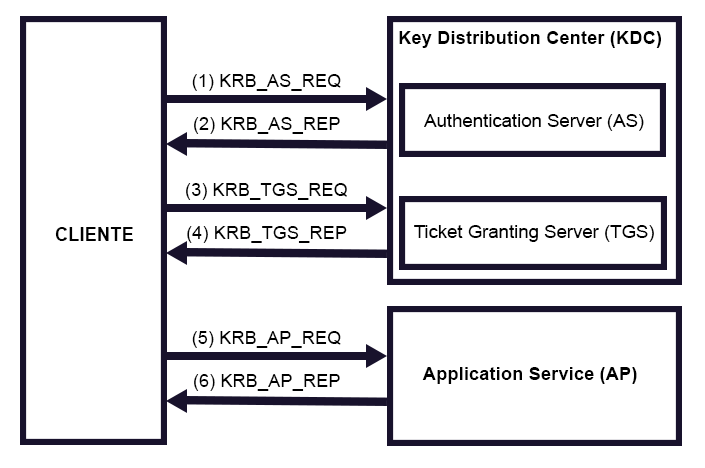
\includegraphics[width=16cm]{Kerberos.png}
\end{center}
\caption{Protocolo de autenticación Kerberos.}
\label{Kerberos}
\end{figure}

\begin{Enumerate}
\item Antes de acceder a un servicio, el c
\end{Enumerate}


























\chapter{Active Directory}
Directotio Activo del inglés {\it Active Directory (AD)}, corresponde a la implementación de un servicio de directorio proporcionado por Microsoft. La finalidad principal de este servicio es la gestión y administración centralizada de los recursos y los usuarios pertenecientes a una red de una empresa u organización. La in\-for\-ma\-ción admisitrada por Active Directory se puede agrupar en tres grupos princiaples: recursos (impresoras), servicios (aplicaciones web, aplicaciones de correo electróncio, bases de datos, etc.) y usuarios (cuentas, credenciales, grupos, etc.). Con esta in\-for\-ma\-ción, es posible crear y adminsitrar dominios, usuarios y todos los objetos englobados dentro de la misma red. En este capítulo se va a introducir los términos generales y conceptos clave y la creación de un laboratorio local que permita la ejecución de los principales ataques sobre Active Directory.

\section{Protocolos y servicios implicados en Active Directory}

\subsubsection{Domain Name System (DNS)}

{\it Domain Name System (DNS)} es el sevicio que proporciona la resolución de nombres de dominio, es decir, resuleve la dirección IP de cada nombre de dominio utilizado en un entorno Active Directory. Este servicio es de gran importancia ya que Active Directory se basa en la resolución de nombres para establecer qué recursos están disponibles a lo largo de una red y dónde se encuentran. 


\subsubsection{Lightweight Directory Access Protocol (LDAP)}

{Lightweight Directory Access Protocol (LDAP)} es un procolo que sirve para acceder a los servicios de directorio. Es utilizado por Active Directory como mecanismo de comunicación entre apliciones y equipos con los servicios que dispone el directorio. Además realiza un seguimiento de los objetos existentes en una red. 


\subsubsection{Server Message Block (SMB)}

{\it Server Message Block (SMB)} es utilizado para el intercambio de archivos a través de un dominio en servicio de Active Directory. Los controladores de dominio utilizan este protocolo para intercambiar Group Policy Objects. 


\section{Términos y conceptos clave}


\subsubsection{Active Directory Domain Services (ADDS)}

{\it Active Directory Domain Services (ADDS)} es el servicio de Active Directory cuando este es intalado en un servidor como por ejemplo Windows Server 2016 ó Windows Server 2019.

\subsubsection{Dominio (Domain)}

Un dominio, del inglés {\it Domain}~\cite{Capitulo4:Domain} es definido como un ``contenedor lógico'', es decir, es una estructura lógica que contiene los siguientes componentes:

\begin{itemize}
\item Una estructura jerárquica para usauarios y grupos en función de los privilegios de los mismos.
\item Servicios (vistos anteriormente) que proveen capacidades de autenticación y autorización.
\item Distintas políticas de seguridad que se aplican a usuarios y objetos.
\item Un registro DNS que identifica inequívocamente el dominio, como puede ser empresa.com, ad.empresa.com. Este nombre será requisito para iniciar sesión en una cuenta de dominio utilizándose como parte del nombre del usuario. 
\end{itemize}

Estos componentes y objetos están almacenados en la base de datos de Active Directory. Se puede considerar un dominio como un límite administrativo de estos objetos. Un dominio puede abarcar diferentes ubicaciones tanto físicas como en red y estar compuesto por una multitud de objetos.

\subsubsection{Árbol (Domain Tree)}

En relación con el término anterior, un árbol del inglés {Domain Tree}, son colecciones de dominios que se agrupan como una estructura jerárquica. Un arbol se le puede considerar como una serie de dominios conectados jerárquicamente a través de usar el mismo espacio de nombres DNS. Un ejemplo sería, si al dominio anterior: empresa.com le añadimos un ``hijo'' denominado recursoshumanos.empresa.com se crea un árbol de dominios compuesto por un dominio padre o root (empresa.com) y un hijo o child (recursoshumanos.empresa.com). Estos dominios forman parte del mismo árbol y se crean automáticamente relaciones de confianza entre ellos. En un Active Directory pueden coexisstir multitud de árboles de dominio diferentes. 

\subsubsection{Bosque (Forest)}
Un bosque, del inglés {\it Forest}, a grandes rasgos es una colección de árboles de dominio que comparten el mismo {\it schema}, misma estructura lógica, {\it global catalog} y configuración. Alguno de estos términos será introducido a continuación. Todos los dominios pertenecientes a un mismo forest, establecen una relación de confianza transitiva. Cabe destacar, que cuando se crea una instacia de Active Directory por primera vez y se crea un dominio también se está creando implícitamente un forest. 

\subsubsection{Schema}

Un {\it schema} en Active Directory se define como a {\it forest-wide template}, es decir, una plantilla aplicable al dominio que define los objetos y propiedades alojados en el Active Directory. Este esquema debe estar bien configurado para evitar comprometer la seguridad de todos los dominios del forest. Para su administración existe un grupo especial denominado {\it Schema Admins} que puede editar y configurar dicho schema. 

\subsubsection{Fully Qualified Domain Name (FQDM)}

Fully Qualified Domain Name (FQDN) es la dirección completa que identifica un host o recurso, este está compuesto por la unión del nombre del host {\it hostname} y el dominio. En el ejemplo anterior, un equipo denominado Cliente01 su FQDN sería Cliente01.empresa.com. 

\subsubsection{Domain Controller (DC)}

Un controlador de dominio, del inglés {\it Domain Controller (DC)}, es la parte fundamental de Active Directory, corresponde a servidores de Windows que contienen la base de datos Active Directory y por lo tanto almacenan toda la información correcpondiente a dominios, domain trees, forests, usuarios, servicieos, etc. 

\subsubsection{Objetos (Objects)}

Todos los elementos alamacenados en una base de datos Active Directory se almacenan en forma de objetos, cada objeto tiene un tipo diferente que le diferencia de otros objetos. Cada objeto almacenado tiene un SID diferente que se utiliza para admitir o denegar el acceso del objeto a un recurso del dominio. Los objetos creados por defecto en cualqueir dominio se pueden agrupar de la siguiente forma: 

\begin{itemize}
\item Unidades organizativas, del inglés {\it Organizational Unit (OU)}. 
\item Usuarios.
\item Ordenadores. 
\item Grupos de usuarios.
\item Contactos.
\item Carpetas compartidas. 
\item Impresoras compartidas.
\end{itemize}

\subsubsection{Organizational Unit (OU)}

Unidades organizativas, del inglés {\it Organizational Unit (OU)} son contenedores de diferentes objetos del mismo dominio como puede ser otros contenedores, cuentas de usuario, grupos, etc. Un administrador del dominio puede crear unidades organizativas y aplicarle diferentes directivas de grupo que se aplicarán a todos los objetos de esta unidad, esto permite una administración más eficiente del Active Directory. 

\subsubsection{Service Principal Name (SPN)}

Un {\it Service Principal Name (SPN)}~\cite{Capitulo4:SPN} es un identificador único asociado a una instacia de un servicio. Los SPN son utilizados por el protocolo de autenticación Kerberos para asociar una instacia de un servicio en concreto con una cuenta de inicio de sesión.  




%----------
%	BIBLIOGRAFÍA
%----------	

%\nocite{*} % Si quieres que aparezcan en la bibliografía todos los documentos que la componen (también los que no estén citados en el texto) descomenta está lína

\clearpage
\addcontentsline{toc}{chapter}{Bibliografía}
%\setquotestyle[english]{british} % Cambiamos el tipo de cita porque en el estilo IEEE se usan las comillas inglesas.
%\printbibliography

\bibliography{Bibliografia/Bibliografia}{}
\bibliographystyle{ieeetr}


%----------
%	ANEXOS
%----------	

% Si tu trabajo incluye anexos, puedes descomentar las siguientes líneas
\chapter*{Instalación Windows Server 2019 (DC01)}
\pagenumbering{gobble} % Las páginas de los anexos no se numeran
\addcontentsline{toc}{chapter}{Anexo 1: Instalación Windows Server 2019 (DC01)}
\textbf{Creación de Máquina Virtual}
\begin{enumerate}
\item Test.
\begin{figure}[H] %[H] para here [b] para bottom [t] para top
\begin{center}
\includegraphics[width=10cm]{DC01/MV1.png}
\end{center}
\end{figure}

\item Test
\begin{figure}[H] %[H] para here [b] para bottom [t] para top
\begin{center}
\includegraphics[width=10cm]{DC01/MV2.png}
\end{center}
\end{figure}

\item Test
\begin{figure}[H] %[H] para here [b] para bottom [t] para top
\begin{center}
\includegraphics[width=10cm]{DC01/MV3.png}
\end{center}
\end{figure}

\item Test
\begin{figure}[H] %[H] para here [b] para bottom [t] para top
\begin{center}
\includegraphics[width=10cm]{DC01/MV4.png}
\end{center}
\end{figure}

\item Test
\begin{figure}[H] %[H] para here [b] para bottom [t] para top
\begin{center}
\includegraphics[width=10cm]{DC01/MV5.png}
\end{center}
\end{figure}

\item Test
\begin{figure}[H] %[H] para here [b] para bottom [t] para top
\begin{center}
\includegraphics[width=10cm]{DC01/MV6.png}
\end{center}
\end{figure}

\item Test
\begin{figure}[H] %[H] para here [b] para bottom [t] para top
\begin{center}
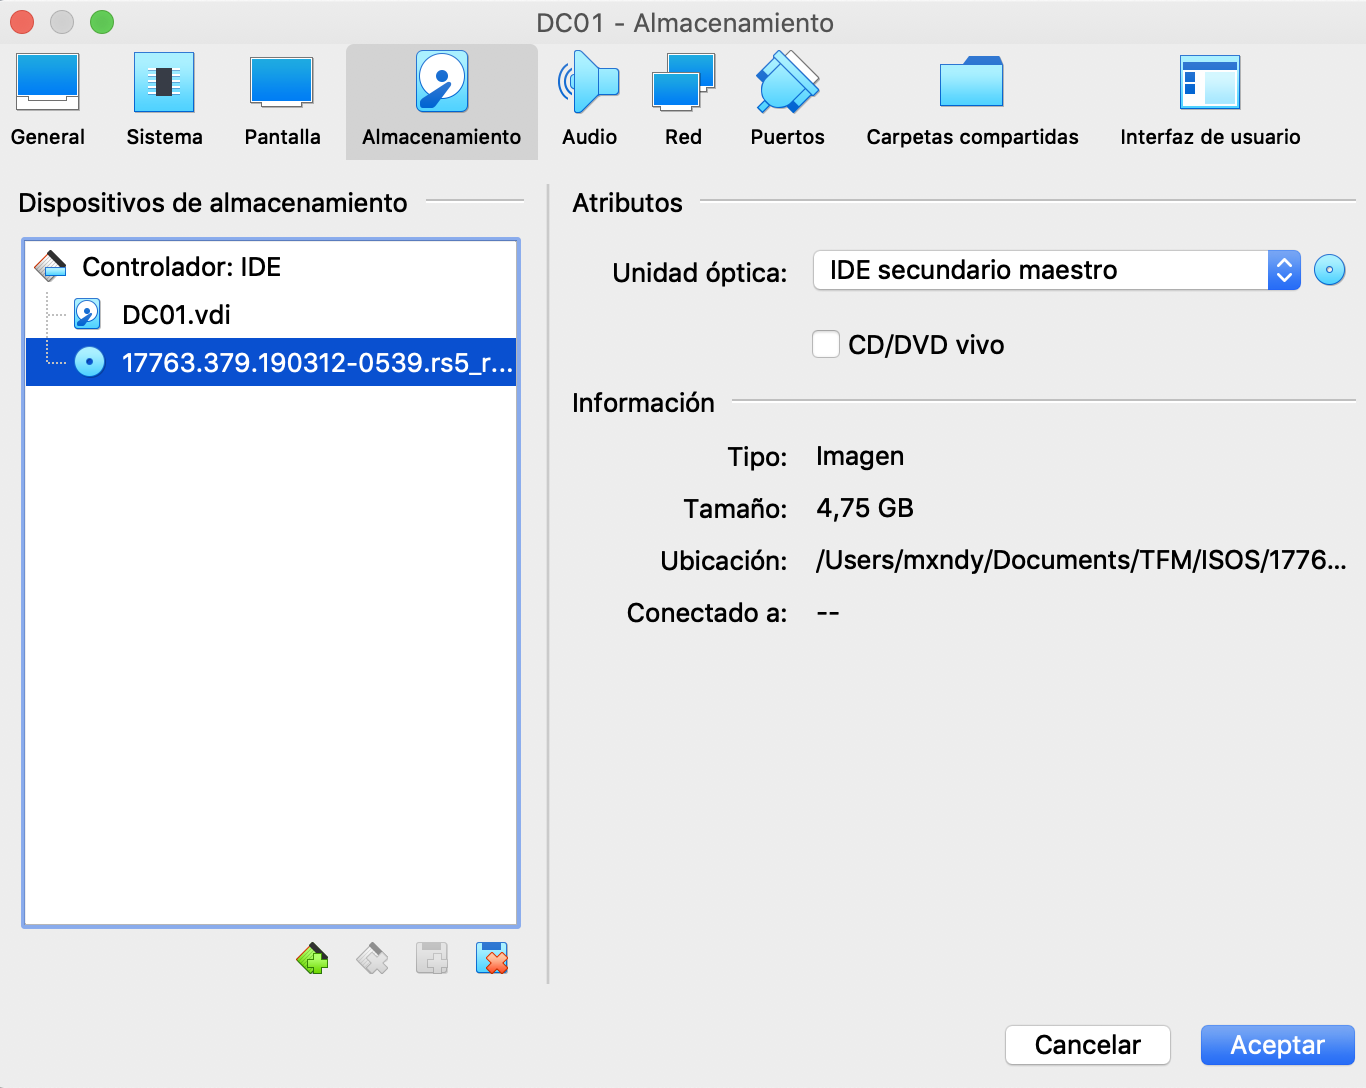
\includegraphics[width=10cm]{DC01/MV7.png}
\end{center}
\end{figure}

\end{enumerate}



\textbf{Instalación}

\begin{enumerate}
\item Una vez creada la máquina virtual se ejecuta la instacia y se procede a la instalación.
\item En primer lugar, se elige el idioma y el teclado a utilizar. En este caso se ha utilizado la imagen (iso) de Windows Server 2019 en inglés: English (United States) y el teclado en español: Spanish (Spain, International Sort) y spanish como método de entrada.

\begin{figure}[H] %[H] para here [b] para bottom [t] para top
\begin{center}
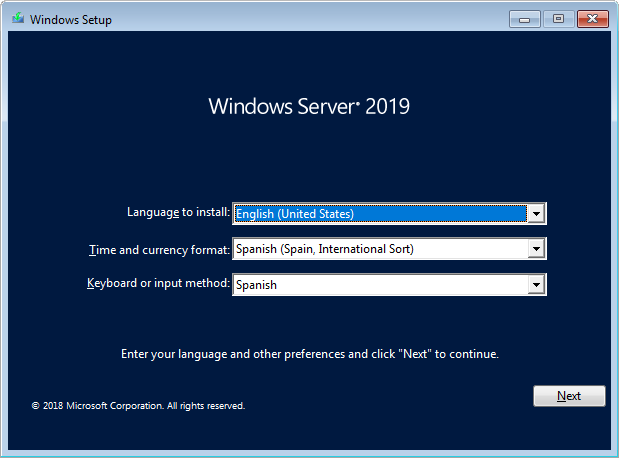
\includegraphics[width=10cm]{DC01/Instalacion1.png}
\end{center}
\end{figure}

\item Se empieza con la instalación pulsando en ``Install Now''.

\begin{figure}[H] %[H] para here [b] para bottom [t] para top
\begin{center}
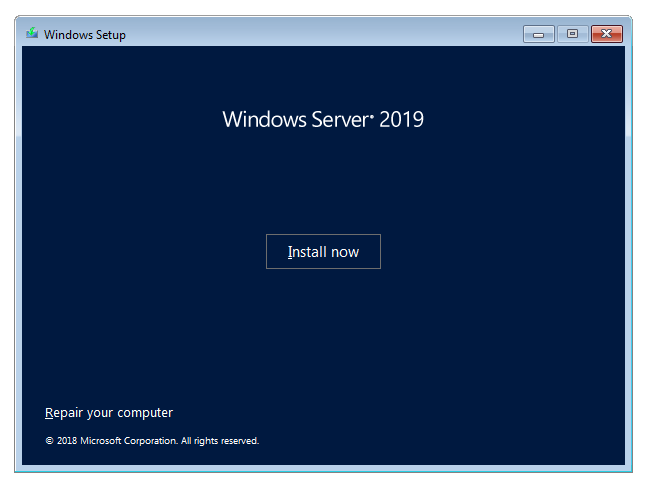
\includegraphics[width=10cm]{DC01/Instalacion2.png}
\end{center}
\end{figure}


\item Test

\begin{figure}[H] %[H] para here [b] para bottom [t] para top
\begin{center}
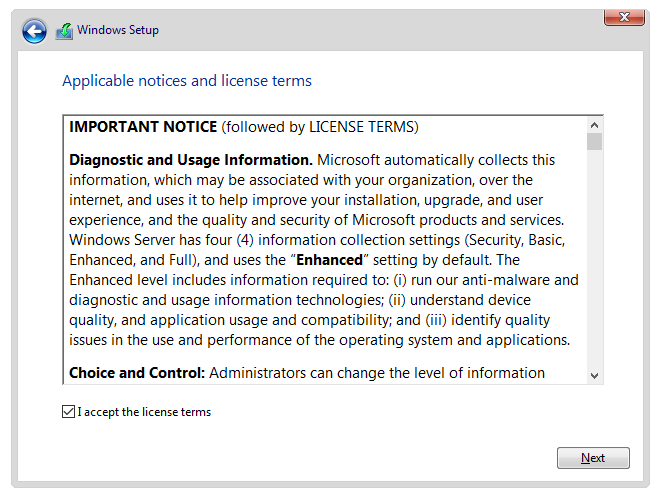
\includegraphics[width=10cm]{DC01/Instalacion3.png}
\end{center}
\end{figure}

\item Test

\begin{figure}[H] %[H] para here [b] para bottom [t] para top
\begin{center}
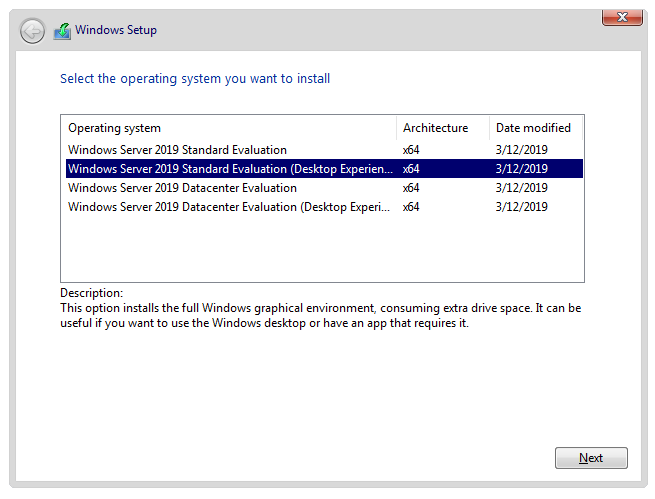
\includegraphics[width=10cm]{DC01/Instalacion4.png}
\end{center}
\end{figure}

\item Test

\begin{figure}[H] %[H] para here [b] para bottom [t] para top
\begin{center}
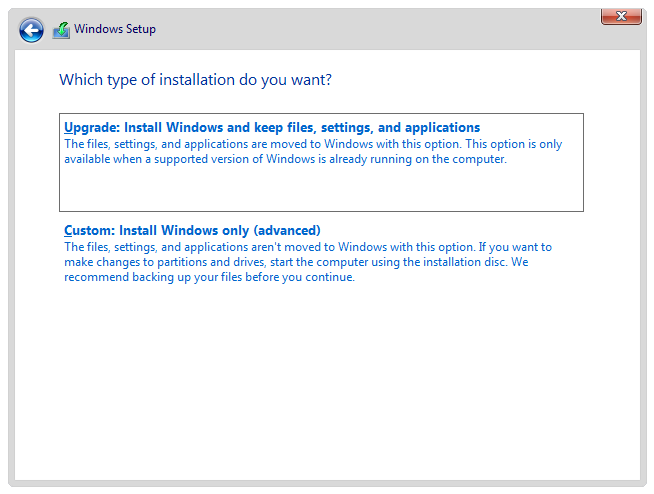
\includegraphics[width=10cm]{DC01/Instalacion5.png}
\end{center}
\end{figure}

\item Test

\begin{figure}[H] %[H] para here [b] para bottom [t] para top
\begin{center}
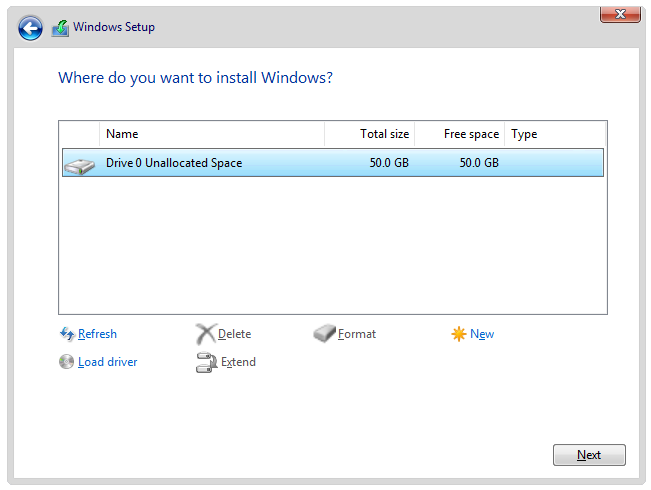
\includegraphics[width=10cm]{DC01/Instalacion6.png}
\end{center}
\end{figure}

\item Test

\begin{figure}[H] %[H] para here [b] para bottom [t] para top
\begin{center}
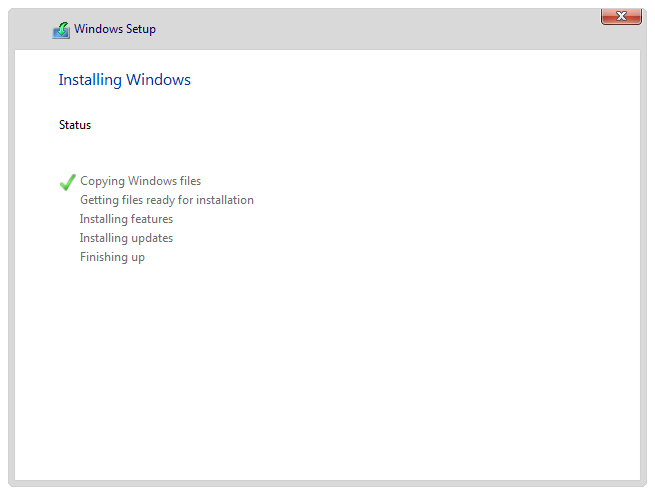
\includegraphics[width=10cm]{DC01/Instalacion7.png}
\end{center}
\end{figure}

\item Test

\begin{figure}[H] %[H] para here [b] para bottom [t] para top
\begin{center}
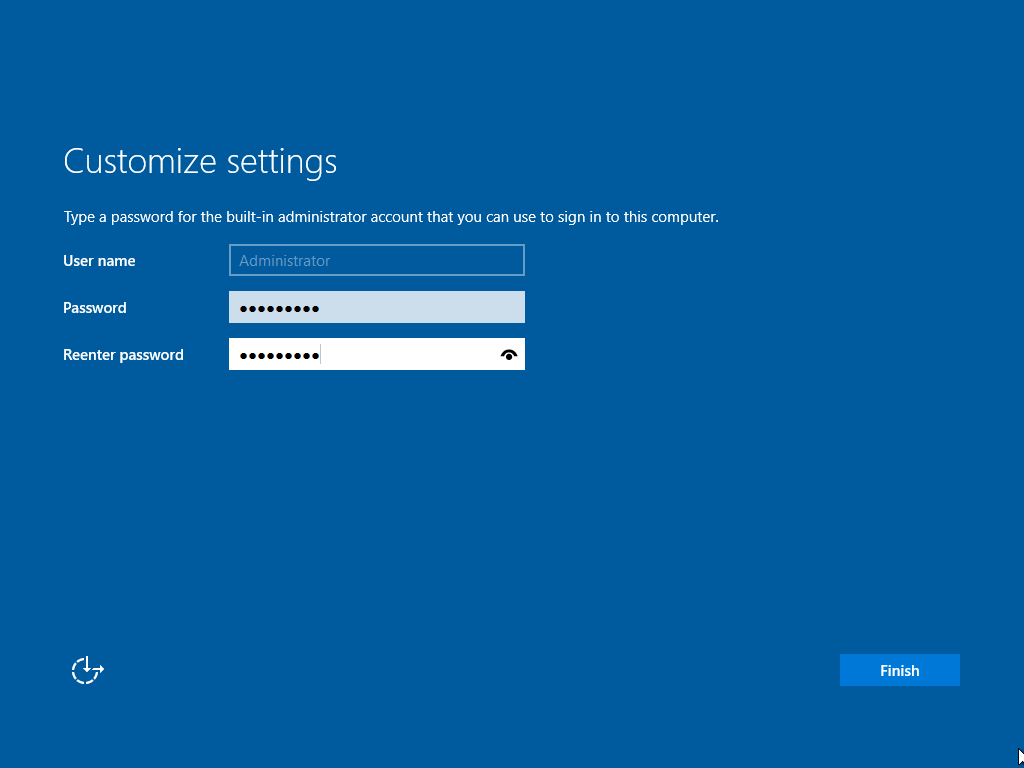
\includegraphics[width=10cm]{DC01/Instalacion8.png}
\end{center}
\end{figure}

\end{enumerate}


\textbf{Actualización}

\begin{enumerate}
\item Test

\begin{figure}[H] %[H] para here [b] para bottom [t] para top
\begin{center}
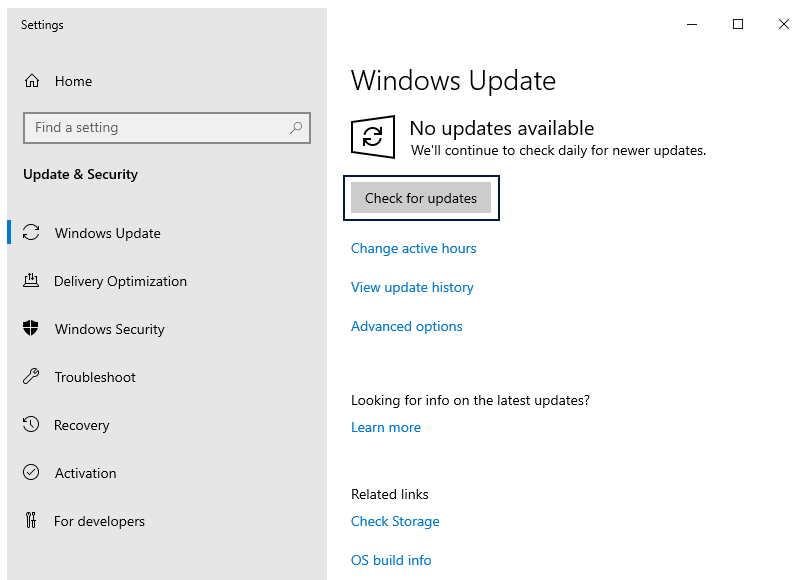
\includegraphics[width=10cm]{DC01/Update1.png}
\end{center}
\end{figure}

\item Test

\begin{figure}[H] %[H] para here [b] para bottom [t] para top
\begin{center}
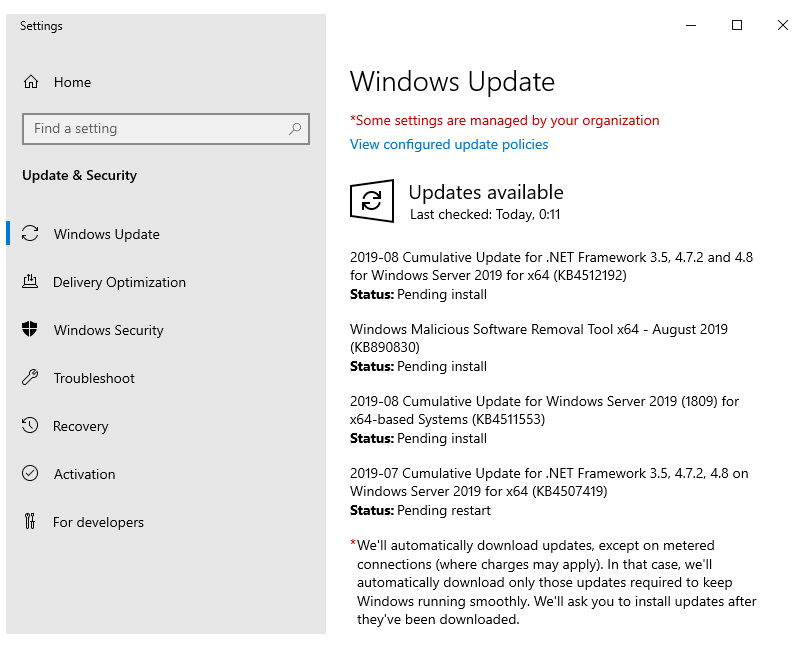
\includegraphics[width=10cm]{DC01/Update2.png}
\end{center}
\end{figure}

\end{enumerate}

\textbf{Configuración}




\chapter*{Instalación Windows 10 Enterprise (Cliente01)}
\addcontentsline{toc}{chapter}{Anexo 2: Instalación Windows 10 Enterprise (Cliente01)}
\textbf{Creación de Máquina Virtual}
\begin{enumerate}

\item En primer lugar, elegimos el nombre de la máquina: \textbf{Cliente01} y el tipo, en este caso se trata de \textbf{Microsoft Windows} versión \textbf{Microsoft Windows 10 (64-bit)}.
\begin{figure}[H] %[H] para here [b] para bottom [t] para top
\begin{center}
\includegraphics[width=10cm]{Cliente01/MV1.png}
\end{center}
\end{figure}

\item En el segundo paso, elegimos la RAM que vamos a destinar a la máquina virtual, aunque el requisito mínimo es de 2GB vamos a destinar 4GB: \textbf{4096 MB} para mejorar la experiencia a la hora de usar esta máquina.
\begin{figure}[H] %[H] para here [b] para bottom [t] para top
\begin{center}
\includegraphics[width=10cm]{Cliente01/MV2.png}
\end{center}
\end{figure}

\item En esta opción, se elige \textbf{Crear un disco duro virtual ahora}.
\begin{figure}[H] %[H] para here [b] para bottom [t] para top
\begin{center}
\includegraphics[width=10cm]{Cliente01/MV3.png}
\end{center}
\end{figure}

\item En cuanto al tipo de disco duro virtual se elige \textbf{VDI (Virtualbox Disk Image)}.
\begin{figure}[H] %[H] para here [b] para bottom [t] para top
\begin{center}
\includegraphics[width=10cm]{Cliente01/MV4.png}
\end{center}
\end{figure}

\item Por último, se ha elegido \textbf{30 GBs} de espacio de disco duro virtual.
\begin{figure}[H] %[H] para here [b] para bottom [t] para top
\begin{center}
\includegraphics[width=10cm]{Cliente01/MV5.png}
\end{center}
\end{figure}

\item Para arrancar la imagen del sistema operativo, hay que seleccionarla desde Con\-fi\-gu\-ra\-ción/\-Almacenamiento de la máquina virtual creada como Unidad Óptica.
\begin{figure}[H] %[H] para here [b] para bottom [t] para top
\begin{center}
\includegraphics[width=10cm]{Cliente01/MV6.png}
\end{center}
\end{figure}




\end{enumerate}
\textbf{Instalación}

\textbf{Actualización}



\chapter*{Instalación Debian 10 (Gateway)}
\addcontentsline{toc}{chapter}{Anexo 3: Instalación Debian 10 (Gateway)}
\textbf{Creación de Máquina Virtual}
\begin{enumerate}

\item En primer lugar, elegimos el nombre de la máquina: \textbf{Gateway} y el tipo, en este caso se trata de \textbf{Linux} versión \textbf{Debian (64-bit)}.
\begin{figure}[H] %[H] para here [b] para bottom [t] para top
\begin{center}
\includegraphics[width=10cm]{Gateway/MV1.png}
\end{center}
\end{figure}

\item En el segundo paso, elegimos la RAM que vamos a destinar a la máquina virtual, al tratarse de un Debian sin entorno gráfico no es necesario destinarle muchos requisos por lo que elegimos 1GB: \textbf{1024 MB}.
\begin{figure}[H] %[H] para here [b] para bottom [t] para top
\begin{center}
\includegraphics[width=10cm]{Gateway/MV2.png}
\end{center}
\end{figure}

\item En esta opción, se elige \textbf{Crear un disco duro virtual ahora}.
\begin{figure}[H] %[H] para here [b] para bottom [t] para top
\begin{center}
\includegraphics[width=10cm]{Gateway/MV3.png}
\end{center}
\end{figure}

\item En cuanto al tipo de disco duro virtual se elige \textbf{VDI (Virtualbox Disk Image)}.
\begin{figure}[H] %[H] para here [b] para bottom [t] para top
\begin{center}
\includegraphics[width=10cm]{Gateway/MV4.png}
\end{center}
\end{figure}

\item Por último, se ha elegido \textbf{10 GBs} de espacio de disco duro virtual.
\begin{figure}[H] %[H] para here [b] para bottom [t] para top
\begin{center}
\includegraphics[width=10cm]{Gateway/MV5.png}
\end{center}
\end{figure}

\item Para arrancar la imagen del sistema operativo, hay que seleccionarla desde Con\-fi\-gu\-ra\-ción/\-Almacenamiento de la máquina virtual creada como Unidad Óptica.
\begin{figure}[H] %[H] para here [b] para bottom [t] para top
\begin{center}
\includegraphics[width=10cm]{Gateway/MV6.png}
\end{center}
\end{figure}




\end{enumerate}
\textbf{Instalación}

\textbf{Actualización}



\chapter*{Instalación Kali Linux 2019.3 (Atacante01)}
\addcontentsline{toc}{chapter}{Anexo 4: Instalación Kali Linux 2019.3 (Atacante01)}
\textbf{Creación de Máquina Virtual}
\begin{enumerate}

\item En primer lugar, elegimos el nombre de la máquina: \textbf{Atacante01} y el tipo, en este caso se trata de \textbf{Linux} versión Kali Linux 2019.3, como esta opción no está disponible elegimos \textbf{Other Linux (64-bit)}.
\begin{figure}[H] %[H] para here [b] para bottom [t] para top
\begin{center}
\includegraphics[width=10cm]{Atacante01/MV1.png}
\end{center}
\end{figure}

\item En el segundo paso, elegimos la RAM que vamos a destinar a la máquina virtual, al tratarse de la máquina donde se van a realizar las pruebas se destinan 4GB: \textbf{4096 MB}.
\begin{figure}[H] %[H] para here [b] para bottom [t] para top
\begin{center}
\includegraphics[width=10cm]{Atacante01/MV2.png}
\end{center}
\end{figure}

\item En esta opción, se elige \textbf{Crear un disco duro virtual ahora}.
\begin{figure}[H] %[H] para here [b] para bottom [t] para top
\begin{center}
\includegraphics[width=10cm]{Atacante01/MV3.png}
\end{center}
\end{figure}

\item En cuanto al tipo de disco duro virtual se elige \textbf{VDI (Virtualbox Disk Image)}.
\begin{figure}[H] %[H] para here [b] para bottom [t] para top
\begin{center}
\includegraphics[width=10cm]{Atacante01/MV4.png}
\end{center}
\end{figure}

\item Por último, se ha elegido \textbf{15 GBs} de espacio de disco duro virtual.
\begin{figure}[H] %[H] para here [b] para bottom [t] para top
\begin{center}
\includegraphics[width=10cm]{Atacante01/MV5.png}
\end{center}
\end{figure}

\item Para arrancar la imagen del sistema operativo, hay que seleccionarla desde Con\-fi\-gu\-ra\-ción/\-Almacenamiento de la máquina virtual creada como Unidad Óptica.
\begin{figure}[H] %[H] para here [b] para bottom [t] para top
\begin{center}
\includegraphics[width=10cm]{Atacante01/MV6.png}
\end{center}
\end{figure}




\end{enumerate}
\textbf{Instalación}

\textbf{Actualización}




\end{document}
